%%%%%%%%%%%%%%%%%%%%%%%%%%%%%%%%%%%%%%%%%
% Beamer Presentation
% LaTeX Template
% Version 1.0 (10/11/12)
%
% This template has been downloaded from:
% http://www.LaTeXTemplates.com
%
% License:
% CC BY-NC-SA 3.0 (http://creativecommons.org/licenses/by-nc-sa/3.0/)
%
%%%%%%%%%%%%%%%%%%%%%%%%%%%%%%%%%%%%%%%%%

%----------------------------------------------------------------------------------------
%	PACKAGES AND THEMES
%----------------------------------------------------------------------------------------


\documentclass{beamer}

\mode<presentation> {

% The Beamer class comes with a number of default slide themes
% which change the colors and layouts of slides. Below this is a list
% of all the themes, uncomment each in turn to see what they look like.

%\usetheme{default}
%\usetheme{AnnArbor}
%\usetheme{Antibes}
%\usetheme{Bergen}
%\usetheme{Berkeley}
%\usetheme{Berlin}
%\usetheme{Boadilla}
%\usetheme{CambridgeUS}
%\usetheme{Copenhagen}
%\usetheme{Darmstadt}
%\usetheme{Dresden}
%\usetheme{Frankfurt}
%\usetheme{Goettingen}
%\usetheme{Hannover}
%\usetheme{Ilmenau}
%\usetheme{JuanLesPins}
%\usetheme{Luebeck}
\usetheme{Madrid}
%\usetheme{Malmoe}
%\usetheme{Marburg}
%\usetheme{Montpellier}
%\usetheme{PaloAlto}
%\usetheme{Pittsburgh}
%\usetheme{Rochester}
%\usetheme{Singapore}
%\usetheme{Szeged}
%\usetheme{Warsaw}

% As well as themes, the Beamer class has a number of color themes
% for any slide theme. Uncomment each of these in turn to see how it
% changes the colors of your current slide theme.

%\usecolortheme{albatross}
%\usecolortheme{beaver}
%\usecolortheme{beetle}
%\usecolortheme{crane}
%\usecolortheme{dolphin}
%\usecolortheme{dove}
%\usecolortheme{fly}
%\usecolortheme{lily}
%\usecolortheme{orchid}
%\usecolortheme{rose}
%\usecolortheme{seagull}
%\usecolortheme{seahorse}
%\usecolortheme{whale}
%\usecolortheme{wolverine}

%\setbeamertemplate{footline} % To remove the footer line in all slides uncomment this line
%\setbeamertemplate{footline}[page number] % To replace the footer line in all slides with a simple slide count uncomment this line

%\setbeamertemplate{navigation symbols}{} % To remove the navigation symbols from the bottom of all slides uncomment this line
}

\usepackage{graphicx} % Allows including images
\usepackage{booktabs} % Allows the use of \toprule, \midrule and \bottomrule in tables
\usepackage{bm}
\usepackage{url}


%----------------------------------------------------------------------------------------
%	TITLE PAGE
%----------------------------------------------------------------------------------------

\title[Short title]{DISCUSSION LOG} % The short title appears at the bottom of every slide, the full title is only on the title page

\author{Sikang Yan} % Your name
\institute[TUK] % Your institution as it will appear on the bottom of every slide, may be shorthand to save space
{
University of Kaiserslautern \\ % Your institution for the title page
\medskip
\textit{yan@rhrk.uni-kl.de} % Your email address
}
\date{\today} % Date, can be changed to a custom date

\begin{document}

\begin{frame}
\titlepage % Print the title page as the first slide
\end{frame}

%------------------------------------------------

\begin{frame}
\frametitle{THEORY}
In our cloth simulation, we follow the precedure written by Rohmer et al..


We consider to begin with the \emph{Defomation gradient} $\mathbf{F}$, which is defined by
\begin{align}
\mathbf{F} = \dfrac{\partial\mathbf{x}}{\partial\mathbf{X}},  
\end{align}
where the $\mathbf{x}$ denotes the deformed vector and the $\mathbf{X}$ denotes the reference vector.


Since we have no further information about the mapping from $\mathbf{X}$ to 
$\mathbf{x}$, we use the vector $\big(\mathbf{u_1},\mathbf{u_2}\big)$ and $\big(\overline{\mathbf{u_1}},\overline{\mathbf{u_2}}\big)$ to approximate the Defomation gradient, which is defined as
\begin{align}
\mathbf{F} = 
\big[\mathbf{u_1},\mathbf{u_2}\big]
\big[\overline{\mathbf{u_1}},\overline{\mathbf{u_2}}\big]^{-1}, 
\label{eq:Defomation_gradient_el} 
\end{align}

Attention should be paid especially:
\begin{itemize}
\item eq.\eqref{eq:Defomation_gradient_el} characrize only the 2D deformation of each triangle.
\item in Rohmer et al. $\mathbf{F}$ is symbolised as $\mathbf{T}$.
\end{itemize}
\end{frame}

%------------------------------------------------

\begin{frame}
\frametitle{KW13}
We provide here our code preceed with concrete data:
\begin{itemize}
\item $faces(i,j)$ is the $j$th vertex of the $i$th triangle, here we choose the $face(0,0),face(0,1),face(0,2)$ as examples and calculate the $VecT$ and $VecR$ for $face(0,0)$.
\end{itemize}
\end{frame}

%------------------------------------------------

\begin{frame}
\begin{block}{$cloth\_vec$}
\begin{align}
VecT=&el_1VertT_1-el_1VertT_2;el_1VertT_1-el_1VertT_3 \\ 
VecR=&el_1VertR_1-el_1VertR_2;el_1VertR_1-el_1VertR_3 
\end{align}
\end{block}
\begin{block}{$cloth\_vec$}
\begin{align}
VecT=&[ 0.771842 \ -0.0144887 \ 6.39045 ]-[ 0.780121 \ -0.0186188 \ 6.37318 ];\\
     &[ 0.771842 \ -0.0144887 \ 6.39045 ]-[ 0.737177\ -0.00912791 \ 6.39292 ] \\
VecR=&[ 0.759919 \ -0.015194 \ 6.38401 ]-[ 0.767822 \ -0.0212492 \ 6.3669  ];\\
	 &[ 0.759919 \-0.015194  \ 6.38401 ]-[ 0.726977 \ -0.00749985 \ 6.38692 ] \\
\end{align}
\end{block}
\end{frame}

%----------------------------------------------------------------------------------------

\begin{frame}
such that
\begin{block}{$cloth\_vec$}
\begin{align}
VecT=&[ -0.0079  \  0.0061 \  0.0171 \ 0.0329 \ -0.0077 \ -0.0029  ];\\ 
VecR=&[ -0.0083  \  0.0041 \  0.0173 \ 0.0347 \ -0.0054 \ -0.0025  ];\\
\end{align}
\end{block} 
where the first 3 entries of $VecR$ is the vector $\mathbf{u_1}$ and the last 3 entries of $VecR$ is the vector $\mathbf{u_2}$. $VecT$ analogiously.
\end{frame}

%----------------------------------------------------------------------------------------

\begin{frame}
\begin{block}{$cloth\_eig\_2D$}
we use here $Eigen::Map$ to transform the vector $VecT$ and $VecR$ to $2*2$ 2D deformation gradient $\mathbf{F}$.
\begin{align}
\mathbf{F}
=
\biggl[
\begin{matrix}
   -0.0083 & 0.0347 \\
   0.0041 & -0.0054 \\
\end{matrix}
\biggr]
\biggl[
\begin{matrix}
   -0.0079 & 0.0329 \\
   0.0061 & -0.0077 \\
\end{matrix}
\biggr]^{-1}
\end{align} 
\end{block} 
\end{frame}

%----------------------------------------------------------------------------------------

\begin{frame}
hence the $\mathbf{F}$ has a rotation information $\mathbf{R}$ and a stretch information $\mathbf{U}$,
\begin{align}
\mathbf{F}=\mathbf{R}\mathbf{U}.
\end{align}
we use $\mathbf{F}^T\mathbf{F}$ to eliminate the ratotion information to obtain $\det\mathbf{R}=1$ 
\begin{align}
\mathbf{F}^T\mathbf{F}=&
\bigl( \mathbf{R}\mathbf{U} \bigr) ^T\mathbf{R}\mathbf{U} \\
=&\mathbf{U}^T\mathbf{R}^T\mathbf{R}\mathbf{U} \\
=&\mathbf{U}^2 \\
=&\mathbf{C}
\end{align}
and using decomposition, if we have the form
\begin{align}
\mathbf{C} = \lambda_1^2\mathbf{v}_1\mathbf{v}_1^T+\lambda_2^2\mathbf{v}_2\mathbf{v}_2^T
\end{align} 
then we could obtain the $\mathbf{U}$ by applying
\begin{align}
\mathbf{U} = \lambda_1\mathbf{v}_1\mathbf{v}_1^T+\lambda_2\mathbf{v}_2\mathbf{v}_2^T
\label{eq:strech_tensor_diagonalized}
\end{align}
\end{frame}

%----------------------------------------------------------------------------------------

\begin{frame}
\begin{figure}
\centering
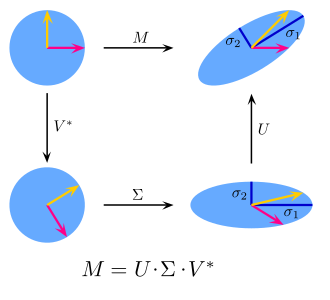
\includegraphics[width=0.5\textwidth]{image//Singular_Value_Decomposition_svd.png}
\caption{Singular Value Decomposition SVD}
\end{figure}
the main backdraw of Rohmer et al. is that this is only applied for 2D problem, thus we need a new algorithm, which can also take the consideration for the vertical deformation. Therefore, the \emph{Kabisch Algorithm} is introduced.
\end{frame}

%----------------------------------------------------------------------------------------

\begin{frame}
\begin{block}{Kabisch Algorithm}
Let $\mathbf{P}$ denotes the points set of template frame, and $\mathbf{Q}$ denotes the points set of reference frame. The \emph{optimal rotation matrix} $\mathbf{R}$ can be calculted as
\begin{align}
\mathbf{R}=\mathbf{V}\biggl[
\begin{matrix}
   1 & 0 &0\\
   0 & 1 &0 \\
   0 & 0 &d
\end{matrix}
\biggr]\mathbf{U}^T
\end{align}
where $\mathbf{V}$ and $\mathbf{U}$ and the \emph{SVD} of \emph{cross-covariance matrix} $\mathbf{H}$, which is determined by
\begin{theorem}[cross-covariance matrix]
\begin{align}
\mathbf{H} =\mathbf{P}^T \mathbf{Q}
\end{align}
\end{theorem}
and $d=\det\mathbf{V}\mathbf{U}^T$
\end{block}
\end{frame}

%----------------------------------------------------------------------------------------

\begin{frame}
The matrix $\mathbf{H}$ is derived from the \emph{orthogonal Procrustes problem}\cite{schonemann1966generalized}. It is defined as the least-squares problem of transforming a given matrix $\mathbf{P}$ into a given matrix $\mathbf{Q}$ by an orthogonal transformation matrix $\mathbf{R}$, such that the sums of squares of the residual matrix $\mathbf{E}=\mathbf{\Omega} \mathbf{P} - \mathbf{Q}$ is a minimum
\begin{align}
\mathbf{R}=\mathop{\arg\min}_{\mathbf{\Omega}} \| \mathbf{\Omega} \mathbf{P} - \mathbf{Q} \|_{F} \quad \mbox{subject to} \quad \mathbf{\Omega}^T\mathbf{\Omega}=\mathbf{I},
\end{align}
where $\| \cdot \|_{F}$ is the Frobenius norm. This problem is equivalent to find the nearest orthogonal matrix $\mathbf{R}$ to a given matrix $\mathbf{H} = \mathbf{P}^T \mathbf{Q}$ \cite{zhang2000flexible}, which most closely maps $\mathbf{P}$ to $\mathbf{Q}$. Thus, we use $\mathbf{H}$ to approximate the deformation gradient $\mathbf{F}$ in Eq. \eqref{eq:deformation_gradient}
\begin{align}
\widetilde{\mathbf{F}} = \mathbf{H}.
\end{align}
\end{frame}

%----------------------------------------------------------------------------------------

\begin{frame}
The cross-covariance matrix discribe the covariance of one process with the other at pairs of time points and measure of similarity. We use therefore the cross-covariance matrix $\mathbf{H}$ to approximate our deformation gradient $\mathbf{F}$.
\begin{figure}
\centering
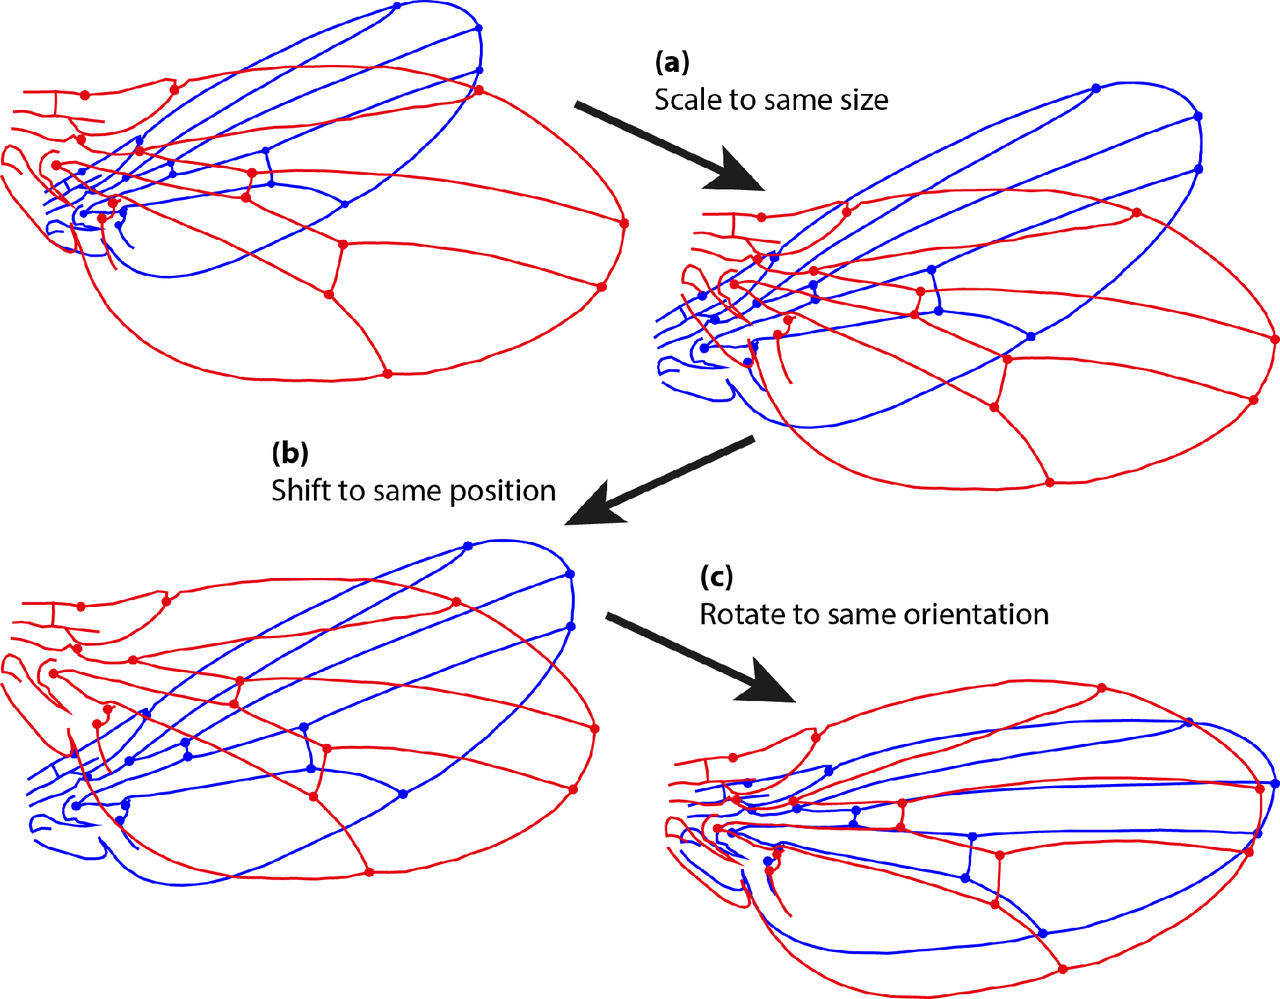
\includegraphics[width=0.5\textwidth]{image//Procrustes_superimposition.png}
\caption{Procrustes superimposition}
\end{figure}
\end{frame}

%----------------------------------------------------------------------------------------

\begin{frame}
Let $i$ be the all index set of the nearst vertice of vertex $I$ in the template frame and $\overline{i}$ be the all index set of the nearst vertice of vertex $I$ in the template frame. Process define
\begin{align}
\mathbf{P}=&\bigg[\begin{matrix}
   \vec{x}_1 \ \vec{y}_1 \ \vec{z}_1\\
   \vec{x}_2 \ \vec{y}_2 \ \vec{z}_2 \\
   \vdots 	\\   
   \vec{x}_N \ \vec{y}_N \ \vec{z}_N \\
\end{matrix}\biggr] \quad 1,2,\dots,N \in i 
\end{align}
\begin{align}
\mathbf{Q}=&\bigg[\begin{matrix}
   \overline{\vec{x}}_1 \ \overline{\vec{y}}_1 \ \overline{\vec{z}}_1\\
   \overline{\vec{x}}_2 \ \overline{\vec{y}}_2 \ \overline{\vec{z}}_2\\
   \vdots 	\\
   \overline{\vec{x}}_N \ \overline{\vec{y}}_N \ \overline{\vec{z}}_N\\
\end{matrix}\biggr] \quad 1,2,\dots,N \in \overline{i} 
\end{align} 
and we apply to obtain the deformation gradient $\mathbf{F}$ of vertex $I$
\begin{align}
\mathbf{F} =\mathbf{P}^T \mathbf{Q}
\end{align}
\end{frame}

%-----------------------------------------------------------------------%

\begin{frame}
Whereas the deformation gradient measures the local deformation, the \emph{spacial velocity gradient} $\mathbf{L}$ describes the rate of deformation, given by
\begin{align}
\mathbf{L} = grad \bm{v} = \dot{\mathbf{F}} \mathbf{F}^{-1},
\end{align}
where $\bm{v}$ denotes the \emph{velocity} of the material point $\mathbf{X}$, and $\dot{\mathbf{F}}$ denotes the material time derivative of deformation gradient $\mathbf{F}$. 

Analogically, we apply the polar decomposition on the spacial velocity gradient $\mathbf{L}$\cite{liu2002continuum}, and obtain
\begin{align}
\mathbf{L} = \mathbf{D}+\mathbf{W}.
\end{align}
Thus, we could decompose the tensor $\mathbf{L}$ into its symmetric part $\mathbf{D}$ and skew-symmetric part $\mathbf{W}$
\begin{align}
\mathbf{D}=&\dfrac{1}{2}(\mathbf{L}+\mathbf{L}^T), \\
\mathbf{W}=&\dfrac{1}{2}(\mathbf{L}-\mathbf{L}^T).
\end{align}
where $\mathbf{D}$ is called the \emph{rate of strain tensor} and $\mathbf{W}$ is called the \emph{rate of rotation tensor}.
\end{frame}

%----------------------------------------------------------------------------------------

\begin{frame}
Assuming $\rm{d}\mathbf{x}$ is a material line element in the current configuration, the rate of change of its length $\dot{\epsilon}_{ii}$ and angle $\dot{\gamma}_{ij}$ is measured by means of $\mathbf{D}$\cite{haupt2013continuum}.
\begin{align}
\dot{\epsilon}_{ii}=&\mathbf{e}_i\mathbf{D}\mathbf{e}_i=D_{ii} \\
\dot{\gamma}_{ij}=&2\mathbf{e}_i\mathbf{D}\mathbf{e}_j=D_{ij}
\end{align}
where $D_{ij}$ are the $ij$-entries of $\mathbf{D}$. Additionally, if $\mathbf{D}$ has the same base ${\mathbf{e_1},\mathbf{e_2},\mathbf{e_3}}$ as in eq.\eqref{eq:strech_tensor_diagonalized}, than
\begin{align}
D_{11}=&\dfrac{\dot{\lambda_1}}{\lambda_1} \\
D_{22}=&\dfrac{\dot{\lambda_2}}{\lambda_3} \\
D_{33}=&\dfrac{\dot{\lambda_2}}{\lambda_3} 
\end{align}

\end{frame}
%----------------------------------------------------------------------------------------

\begin{frame}
\frametitle{KW13}
%use $<boost>$ to collect all ply files name, which are stored in $\_filename$ as well as $\_output$ in $std::vector$. Later I could only pass the index $i$ and $i+1$ for the inputs, and the eigenvector can be calculated automatically and saved.


from 0-2 EigNorm1 8759 NaN, Problrm:: 26278 has -0 eigenvalues, can't be squre. So I use a if(isnan) and define idx=0.

add lambda1,2,3 for all, which is in debug
\end{frame}

%----------------------------------------------------------------------------------------

\begin{frame}
\frametitle{KW14}
save the backsite of clothes using 1-2, 1-3, 1-4. NOt much differences from colormap, need a new color map??? 

save lambda1 for 1,74, they are different, but slightly.

lambda2 has more differences

do also for lambda3
\end{frame}

%----------------------------------------------------------------------------------------

\begin{frame}
\frametitle{KW15}
check color  
run application in loop
consider the kr to ring
1-2 1-3 ...
1-4 2-5 ... 72-75

tensor flow

add neighbor2x


Neo Hook matrial
\end{frame}

%----------------------------------------------------------------------------------------

\begin{frame}
\frametitle{KW15}
please refer
\url{http://web.mit.edu/abeyaratne/Volumes/RCA_Vol_II.pdf} p68-70 $\lambda$ and $\mathbf{D}$ relationship

remedy Neighbor2x

\end{frame}

%----------------------------------------------------------------------------------------

\begin{frame}
$matrix\_example.cpp$

add func to calculate D and L ,think timestep is to small 2-3
\url{http://www.continuummechanics.org/velocitygradient.html}
0.006
1/200

think should use less $2\%$ points for KDtree

\end{frame}

%------------------------------------------------------------------------------

\begin{frame}
\frametitle{KW15}
it is because the date set has isolated points: but I thought it doesn't matter, it influence only the colormap.

thoese points can be deleted during the optimazation.

calculate D using kd-tree.

ask Ali the offical video about clothing deforamtion.

need to be emphasised that we focus on the CR(next time step)
\end{frame}

\begin{frame}
\frametitle{KW15}
LIbreoffice Draw A1

Dornisch Friday. monday presentation

paper send to him

add results

add smooth not finish yet. need to connect opengl and calculation
\end{frame}

\begin{frame}
\frametitle{KW15}
setcolor at end

correct colormap 
\begin{figure}
\centering
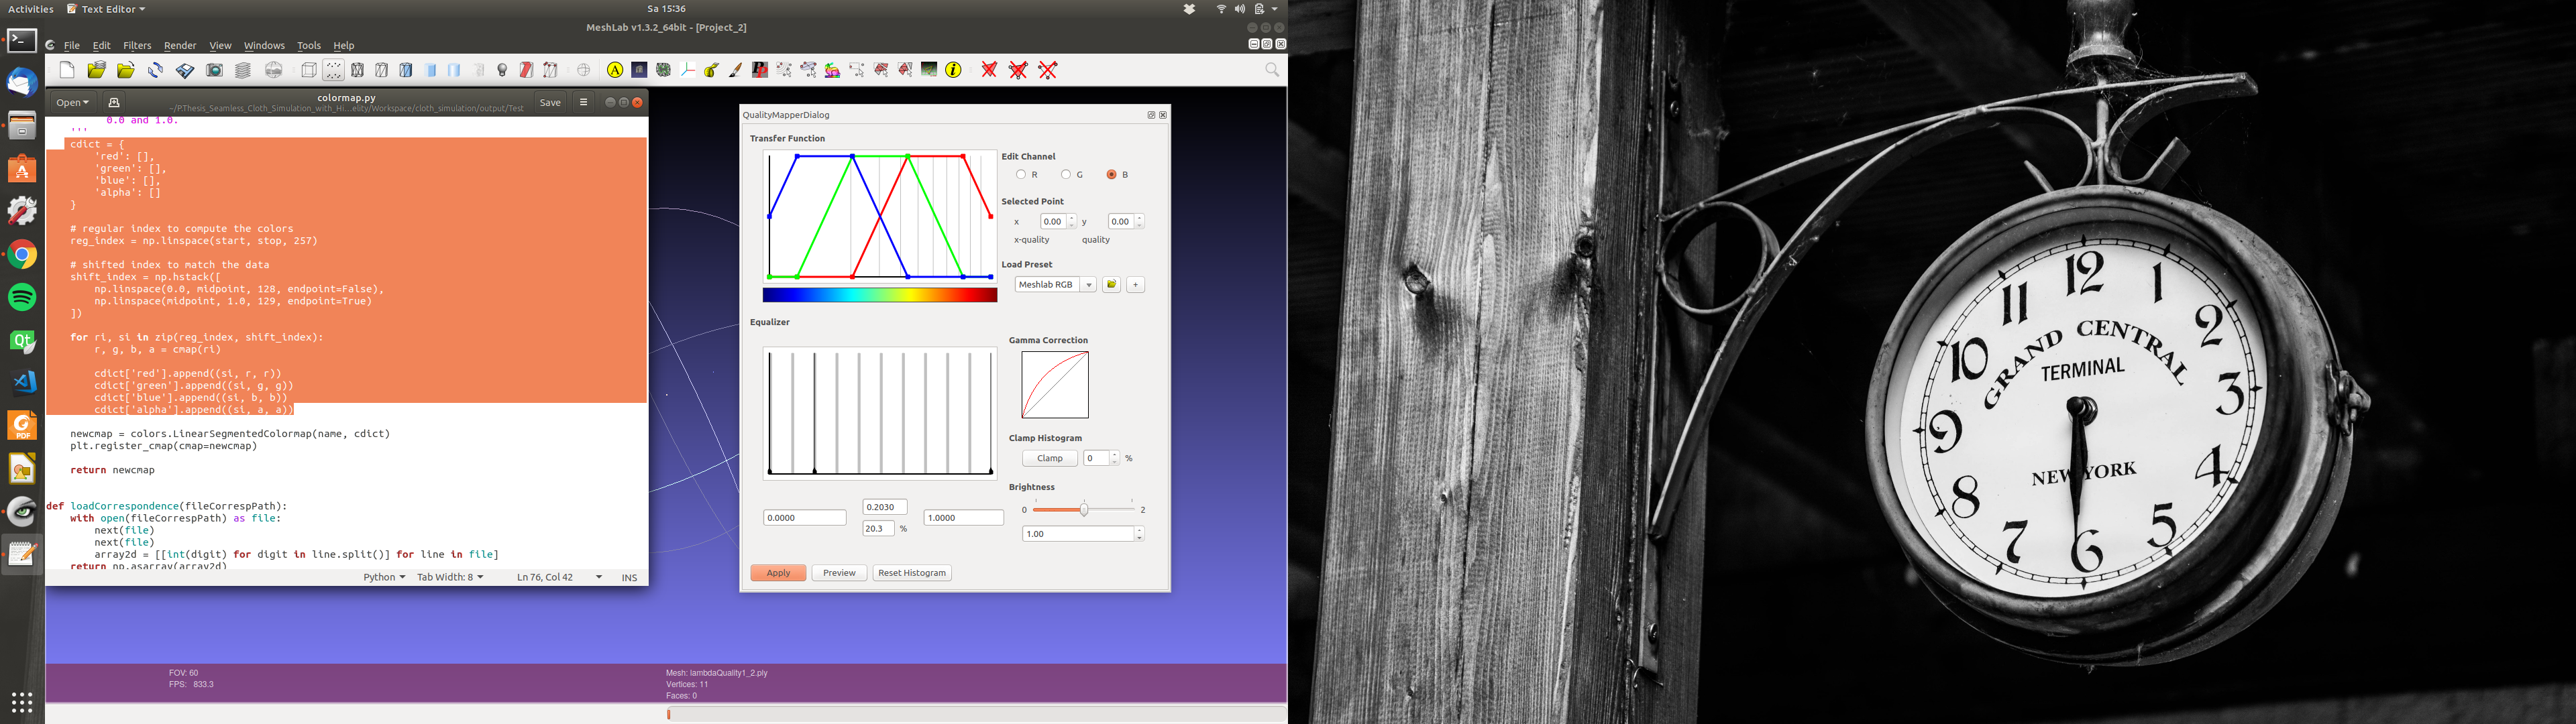
\includegraphics[width=0.5\textwidth]{image//colormap_error.png}
\caption{colormap}
\end{figure}
the erro is by interpolation, how to change it? because meshlab using a unknown function?

dont draw bevor calucution

glMapBuffer

gluPMAPBUFFER
\end{frame}

\begin{frame}
\frametitle{KW15}
add new reulsts using new colormap, have seen red

add defalut color as pink for all vertices

add smooth: problem negative values cannot be root squre...

add colormap for D, based on t not on t+deltaT

tried to pass calculated datas direct to opengl class -> ?, so I directly read the ply file from output. no color? didn't find the glMapBuffer.
\end{frame}


\begin{frame}
IT is actu. a normalizeation (Rohmer)

change Gamma to 1/2.5

$0.1, 0.2, 0.5, 0.75,1, 1.5, 2, 3$ 
\end{frame}

\begin{frame}
new evaluatet

add python for pic, need rotation 

\begin{itemize}
\item tensor density
\url{https://www.revolvy.com/page/Tensor-density}
\item openFoam limited
\end{itemize}
\end{frame}
\begin{frame}
visply

slerp

\url{https://github.com/cmu462/Scotty3D/wiki/Linear-Blend-Skinning}

\begin{figure}
\centering
\includegraphics[width=0.5\textwidth]{image//Muti_pass.png}
\end{figure}

\begin{figure}
\centering
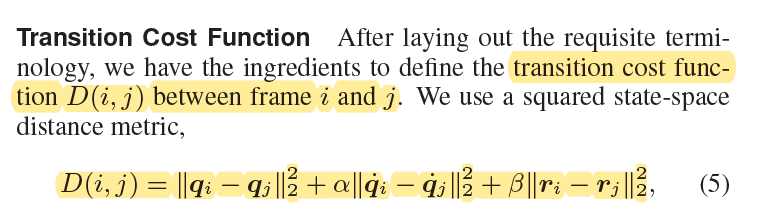
\includegraphics[width=0.5\textwidth]{image//transition_cost_function.PNG}
\end{figure}
\end{frame}

\begin{frame}
\begin{figure}
\centering
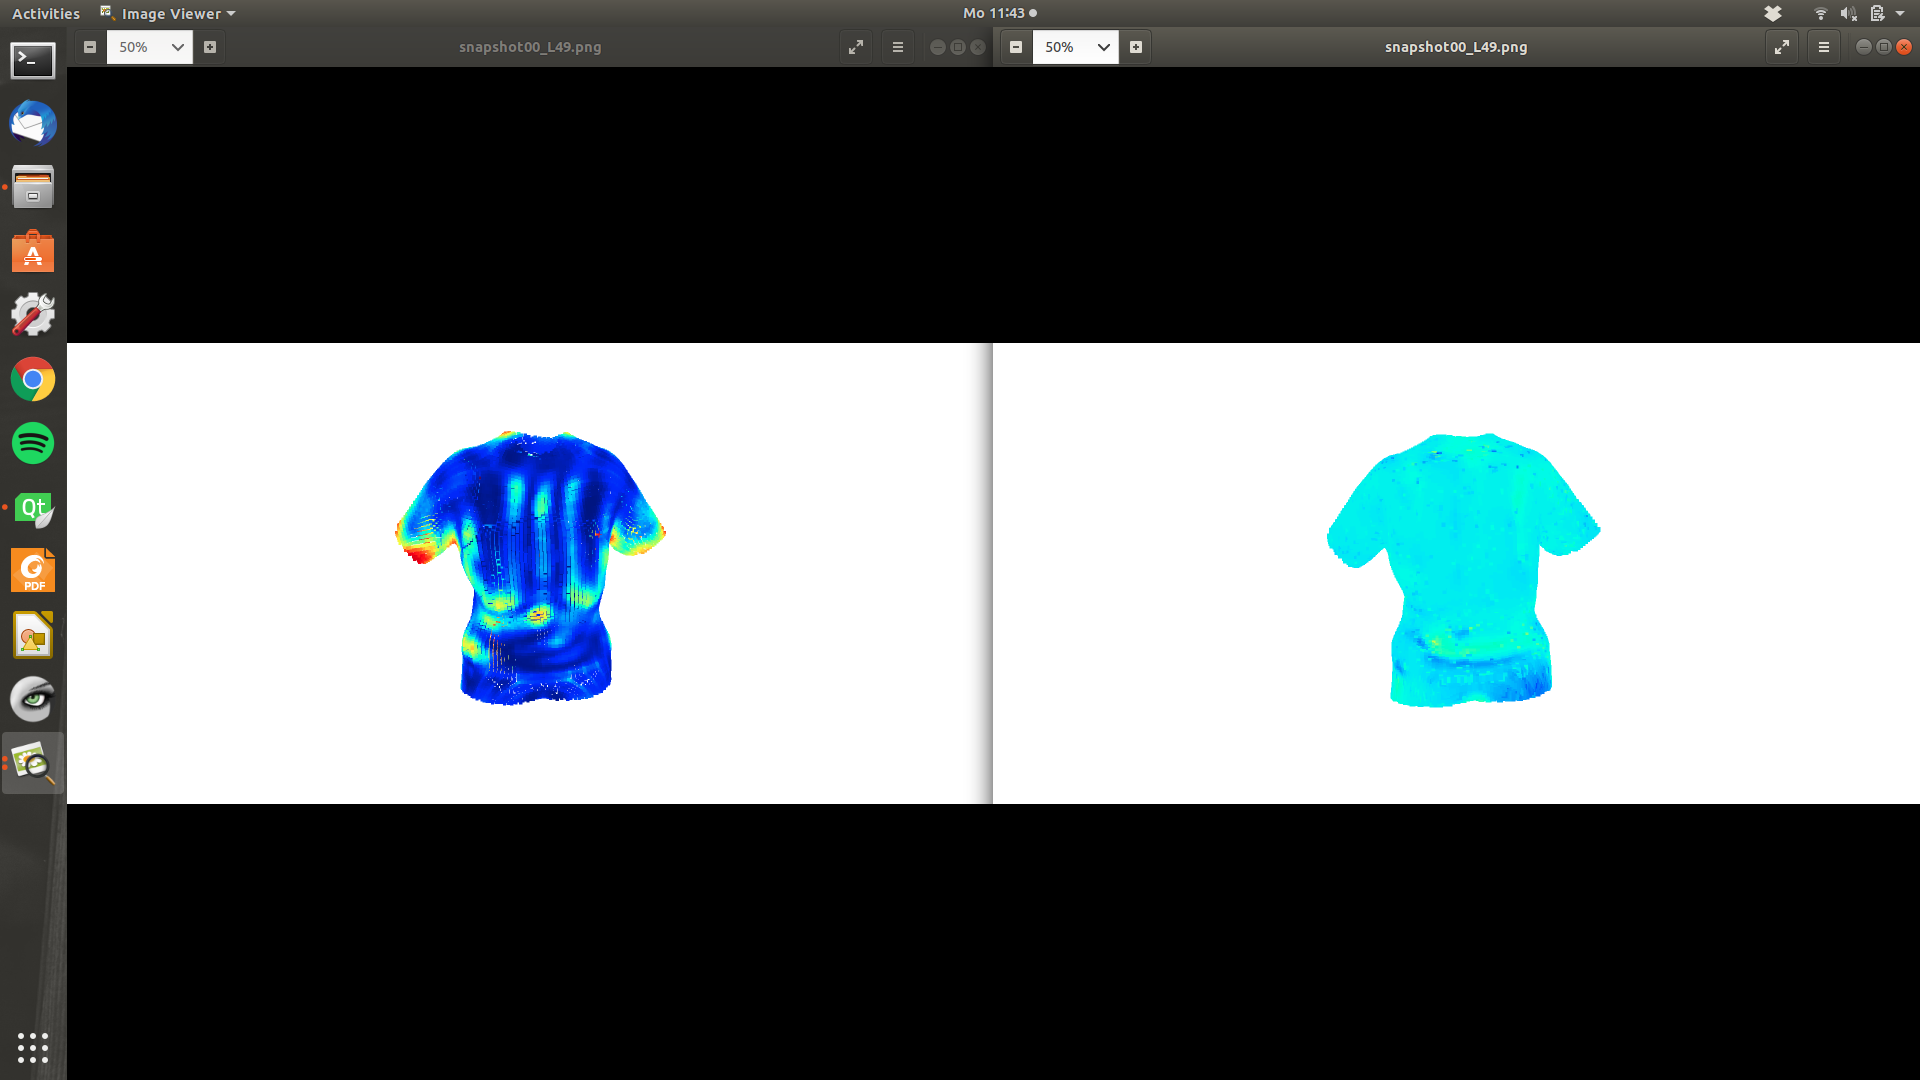
\includegraphics[width=0.5\textwidth]{image//compare.png}
\end{figure}
\end{frame}
\begin{frame}
cannot use QPPP because there are 0 acnnot be inversed, could use kdtree but not good

need binary datas

still negative entries
\end{frame}

\begin{frame}
matrix log / exp

\begin{figure}
\centering
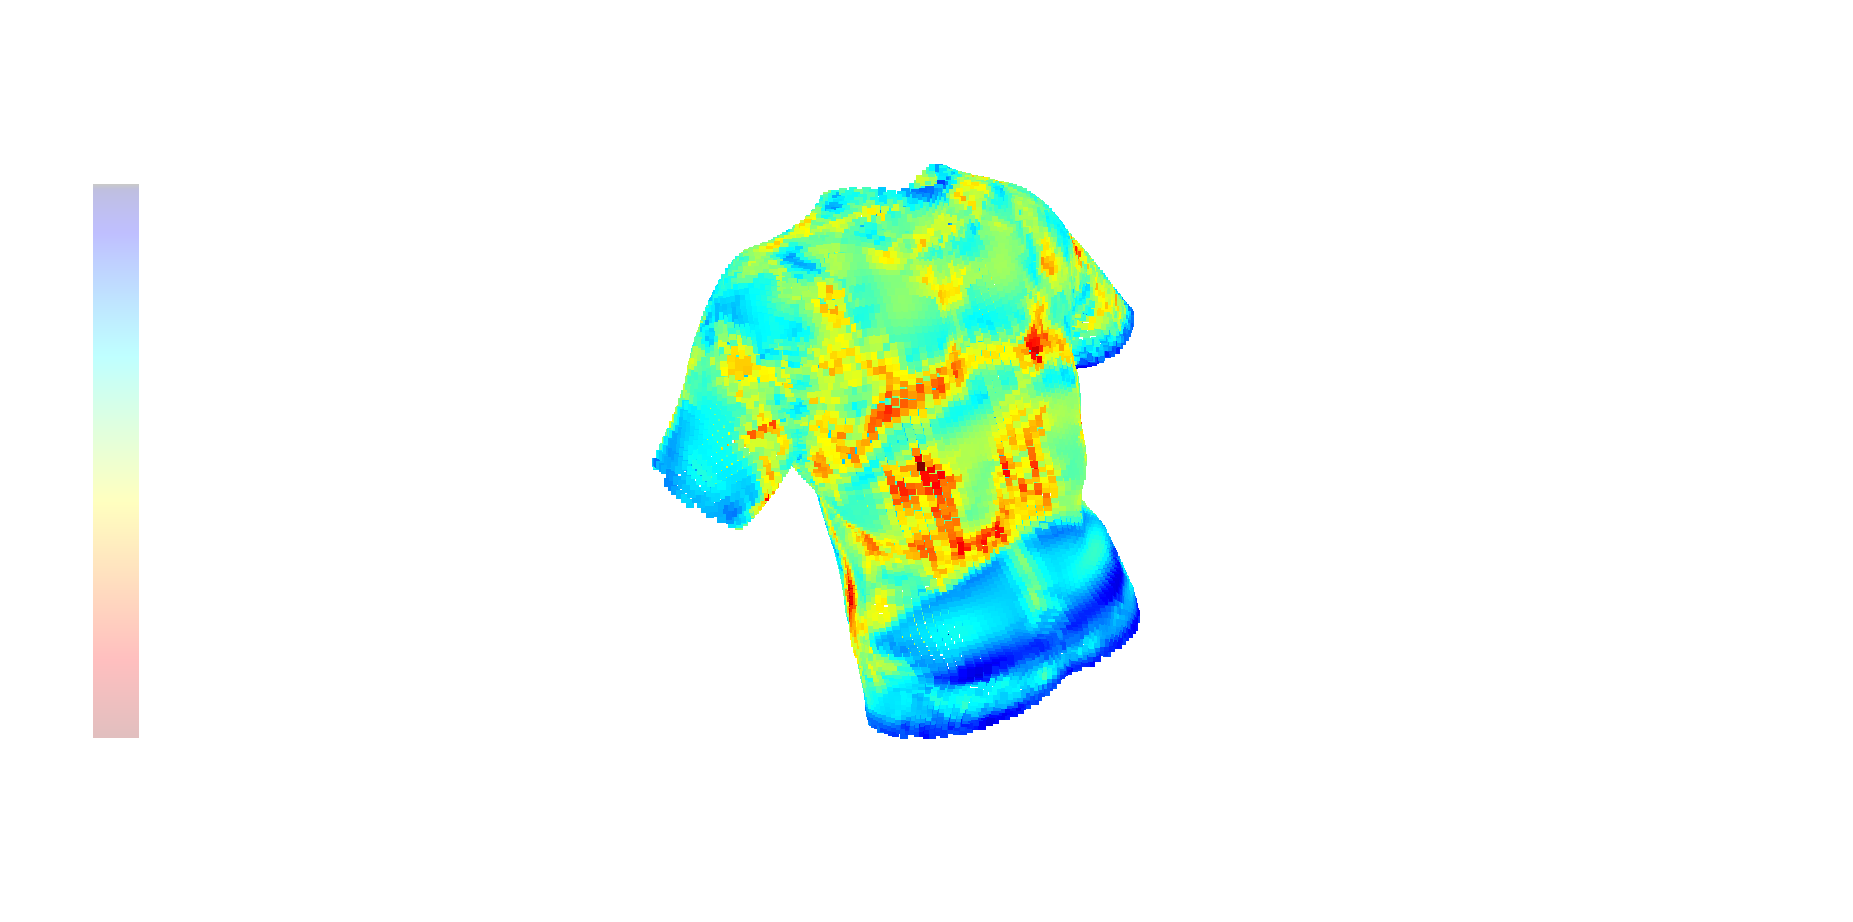
\includegraphics[width=0.5\textwidth]{image//LAMBDA200.png}
\end{figure}

\begin{figure}
\centering
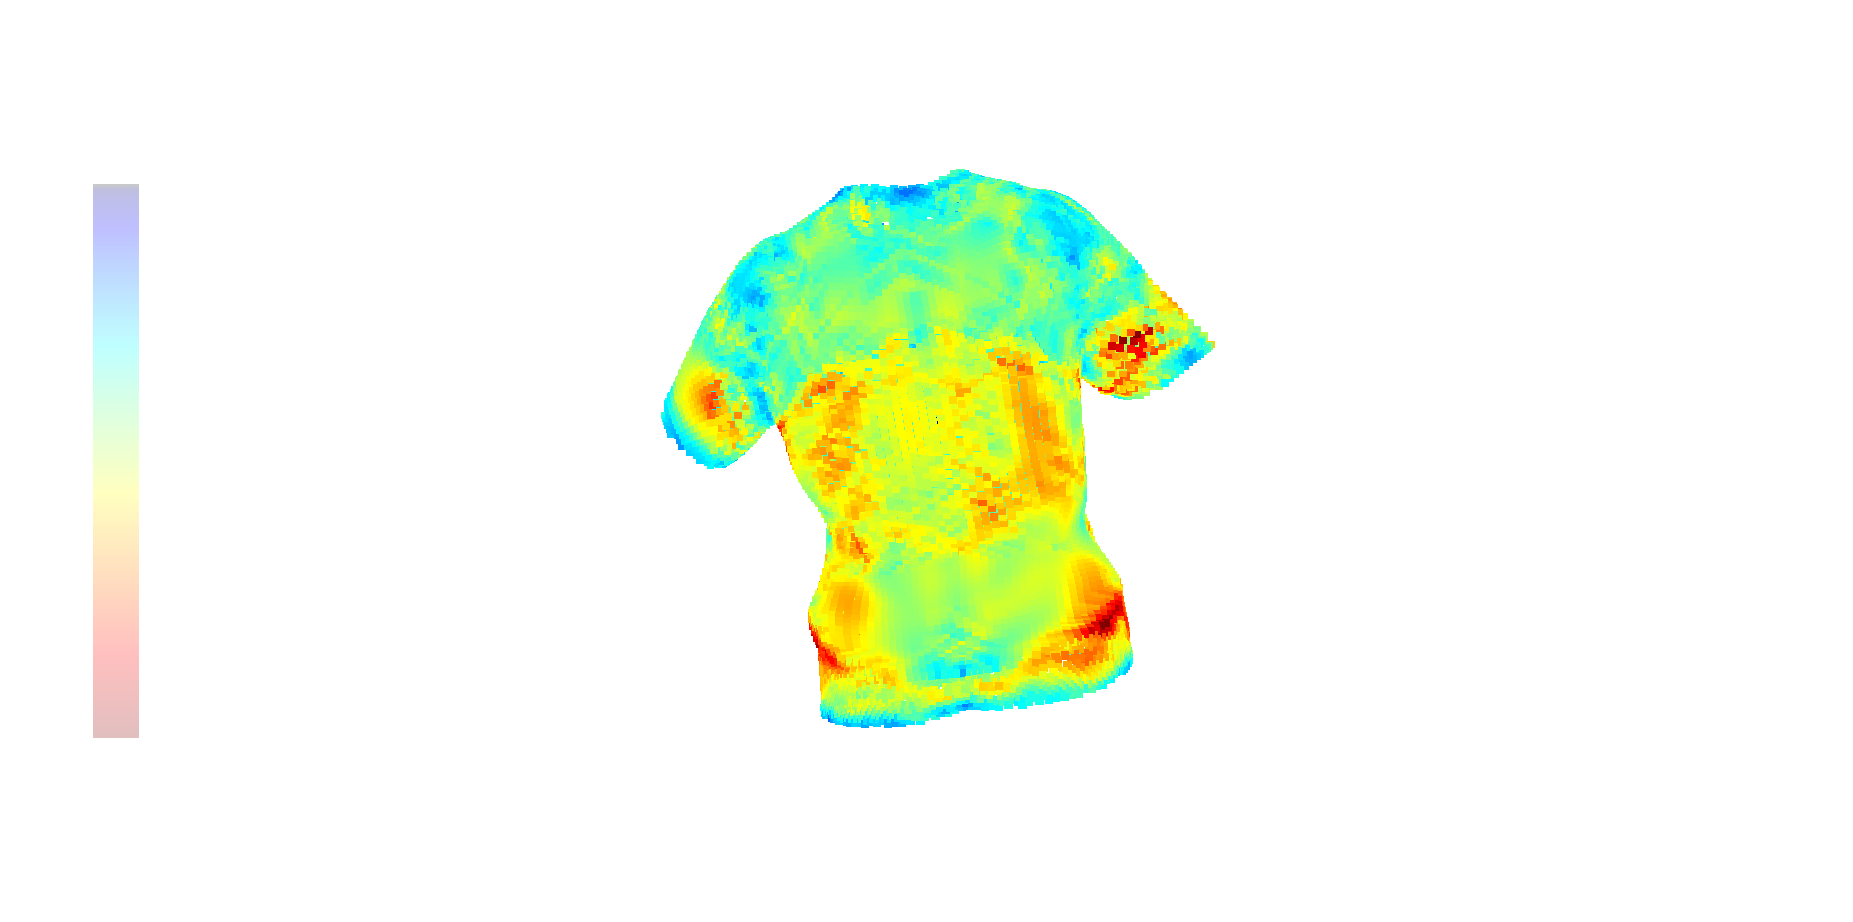
\includegraphics[width=0.5\textwidth]{image//LAMBDA300.png}
\end{figure}

add mapNeighbor method 

add update vertices using kdtree because of 0 of trimesh
\end{frame}

\end{document} 